\subsubsection{World 1: Violations}
The first world presents the most important base functions of the model: it has 2 users and an
officer, all registered with different emails. The users report Violations, which have a position, a set of images
and optionally a ticket. Each local police receives a violation if its position is among the positions of the police itelf,
which form a perimeter around the city.

In each violation there is always at least an image which shows a licence plate that has been read
by the system. All the violations also have a violationType and the police system also exposes accidents along with their type.

\begin{figure}
    \noindent\makebox[\textwidth]{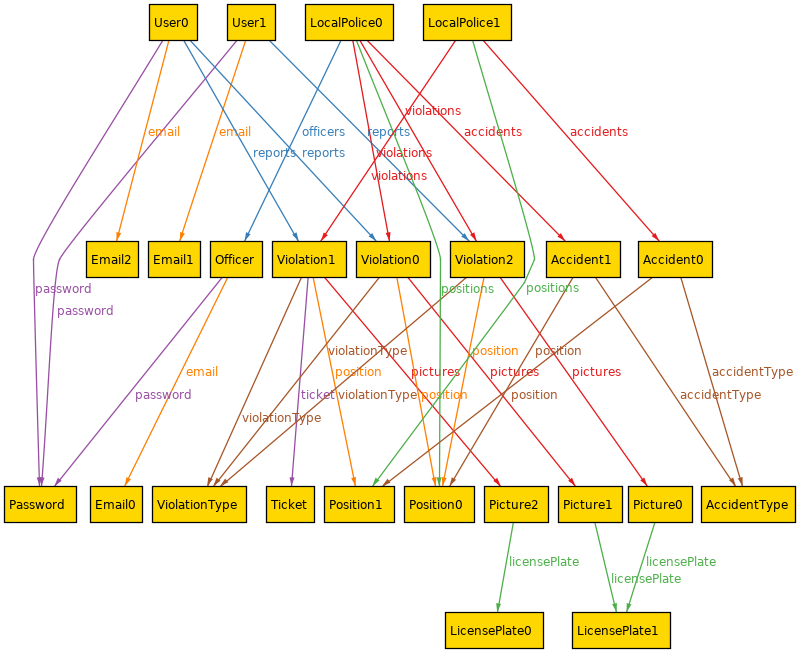
\includegraphics[width=0.95\paperwidth]{images/worlds/world1.png}}
    \caption{World 1 generation in Alloy}
\end{figure}

\subsubsection{World 2: Suggestions}
The second world shows a complete representation of the unsafe areas: each local police system gets signalled by SafeStreet
a series of unsafe areas, which are connected to a position and are always in the police system handling that position.
Each unsafePosition is connected to an unsafeReason, which is itself made by a violationType an accidentType and a suggestion. This is
because the unsafeReasons are inserted by hand by operators using accident and violation categories.

The system detects an unsafe area if there are enough accidents and violations of a certain type in a position, and
suggests a possible solution.

\begin{figure}
    \noindent\makebox[\textwidth]{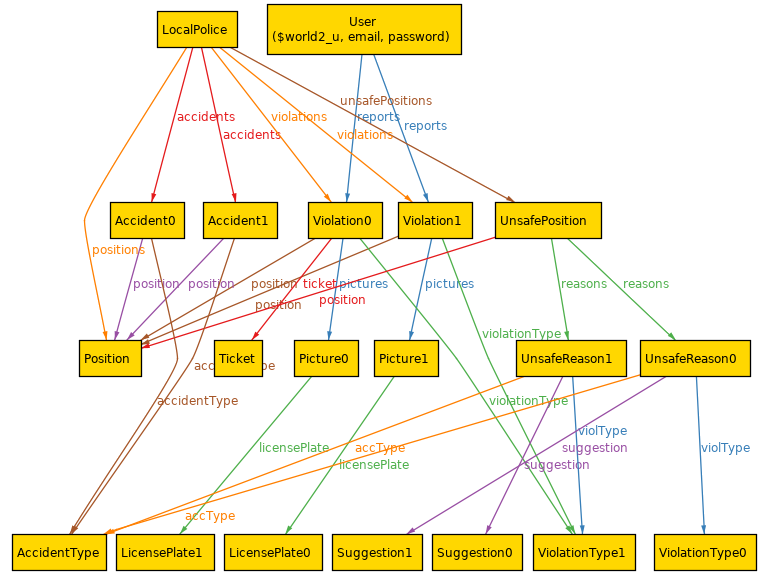
\includegraphics[width=\paperwidth]{images/worlds/world2.png}}
    \caption{World 2 generation in Alloy}
\end{figure}

\subsubsection{World 3: Alteration of information}
This world represents the way in which SafeStreet is sure that from when a violation reaches its systems it
is not altered until it reaches the police systems.

Each Violation is associated to a unique Hash in the Hashes system of SafeStreet, and a ticket is created
only if the hash calculated on the police system matches the one on SafeStreet.

In the picture we can see
that Violations 1 and 3 are confirmedViolations: this means they have the same hashes in the Hashes and PoliceHashes sig.
Also, it is important to notice that the user who issued those violations requested a ticket

\begin{figure}
    \noindent\makebox[\textwidth]{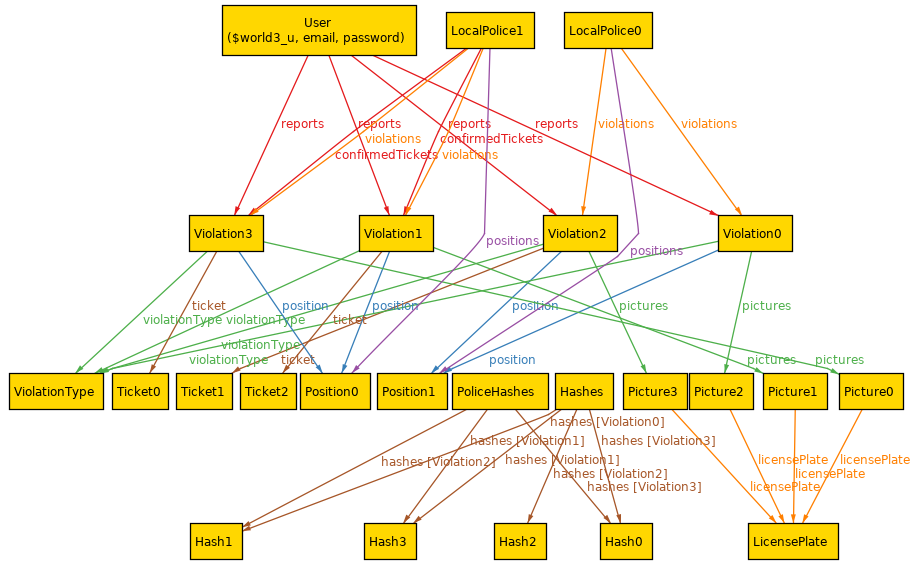
\includegraphics[width=\paperwidth]{images/worlds/world3.png}}
    \caption{World 3 generation in Alloy}
\end{figure}